% IEEE Transactions-style LaTeX template, revised from the uploaded IEEE Access template.
% Main visual changes:
% 1) black title/section styling (no IEEE Access blue title block),
% 2) abstract and index terms remain in the two-column text flow,
% 3) no IEEE Access masthead/header/logo.
%
% Compile locally with: latexmk -pdf access.tex
% Overleaf: set access.tex as the main file and use pdfLaTeX.

\documentclass[journal,twoside]{IEEEtran}

% Basic packages normally supported by TeX Live / Overleaf.
\usepackage{cite}
\usepackage{amsmath,amssymb,amsfonts}
\usepackage{algorithmic}
\usepackage{graphicx}
\usepackage{textcomp}
\usepackage{xcolor}
\usepackage{url}
\usepackage{hyperref}

% Blue citation/link color, consistent with the reference PDF's online version.
% Use hidelinks for a fully black printed manuscript.
\hypersetup{
  colorlinks=true,
  citecolor=blue,
  linkcolor=blue,
  urlcolor=blue
}

% Optional: if your manuscript still uses IEEE Access' \PARstart command,
% this alias keeps it working in IEEEtran.
\providecommand{\PARstart}[2]{\IEEEPARstart{#1}{#2}}

% Optional placeholders for IEEE-style publication metadata.
% Change the journal string, volume/issue/month, and starting page if needed.
\markboth{IEEE Transactions on Cybernetics, Vol. XX, No. X, Month Year}%
{Author \MakeLowercase{\textit{et al.}}: Short Paper Title}
% \setcounter{page}{3263} % Uncomment if a final starting page number is assigned.

\begin{document}

\title{Paper Title in IEEE Transactions Style}

\author{First A. Author, \IEEEmembership{Member, IEEE},
        Second B. Author, and Third C. Author, \IEEEmembership{Fellow, IEEE}%
\thanks{Received XX Month 20XX; revised XX Month 20XX; accepted XX Month 20XX. Date of publication XX Month 20XX; date of current version XX Month 20XX. This work was supported in part by XXXX. (Corresponding author: First A. Author.)}%
\thanks{First A. Author is with the Department of XXX, University XXX, City, Country (e-mail: author1@example.com).}%
\thanks{Second B. Author is with the Department of XXX, University XXX, City, Country (e-mail: author2@example.com).}%
\thanks{Third C. Author is with the Department of XXX, University XXX, City, Country (e-mail: author3@example.com).}%
\thanks{Digital Object Identifier XX.XXXX/XXXX.20XX.XXXXXXX}}

\maketitle

\begin{abstract}
This template is adjusted to resemble the formatting of an IEEE Transactions article rather than an IEEE Access article. The title is typeset in black, without the IEEE Access blue title style. The abstract is placed after \verb|\maketitle|, so it appears in the two-column text area, followed by the index terms. Replace this paragraph with a concise summary of the manuscript, normally written as a single paragraph.
\end{abstract}

\begin{IEEEkeywords}
Index term one, index term two, index term three, index term four.
\end{IEEEkeywords}

\section{Introduction}
\label{sec:introduction}
\IEEEPARstart{T}{his} template uses the standard IEEE Transactions two-column journal layout. It removes the IEEE Access masthead and the blue article-title block. The section headings, title, author block, abstract, and index terms follow the visual logic of the supplied reference paper.

Use \verb|\cite{}| for references, for example \cite{ref1,ref2}. Equations may be written as follows:
\begin{equation}
  E = mc^2.
  \label{eq:einstein}
\end{equation}

\section{Method}
Text, equations, tables, and figures can be added as in a standard IEEE Transactions manuscript. To avoid floats appearing before the abstract on very short sample documents, the figure example is left as a commented block below.

% \begin{figure}[!t]
%   \centering
%   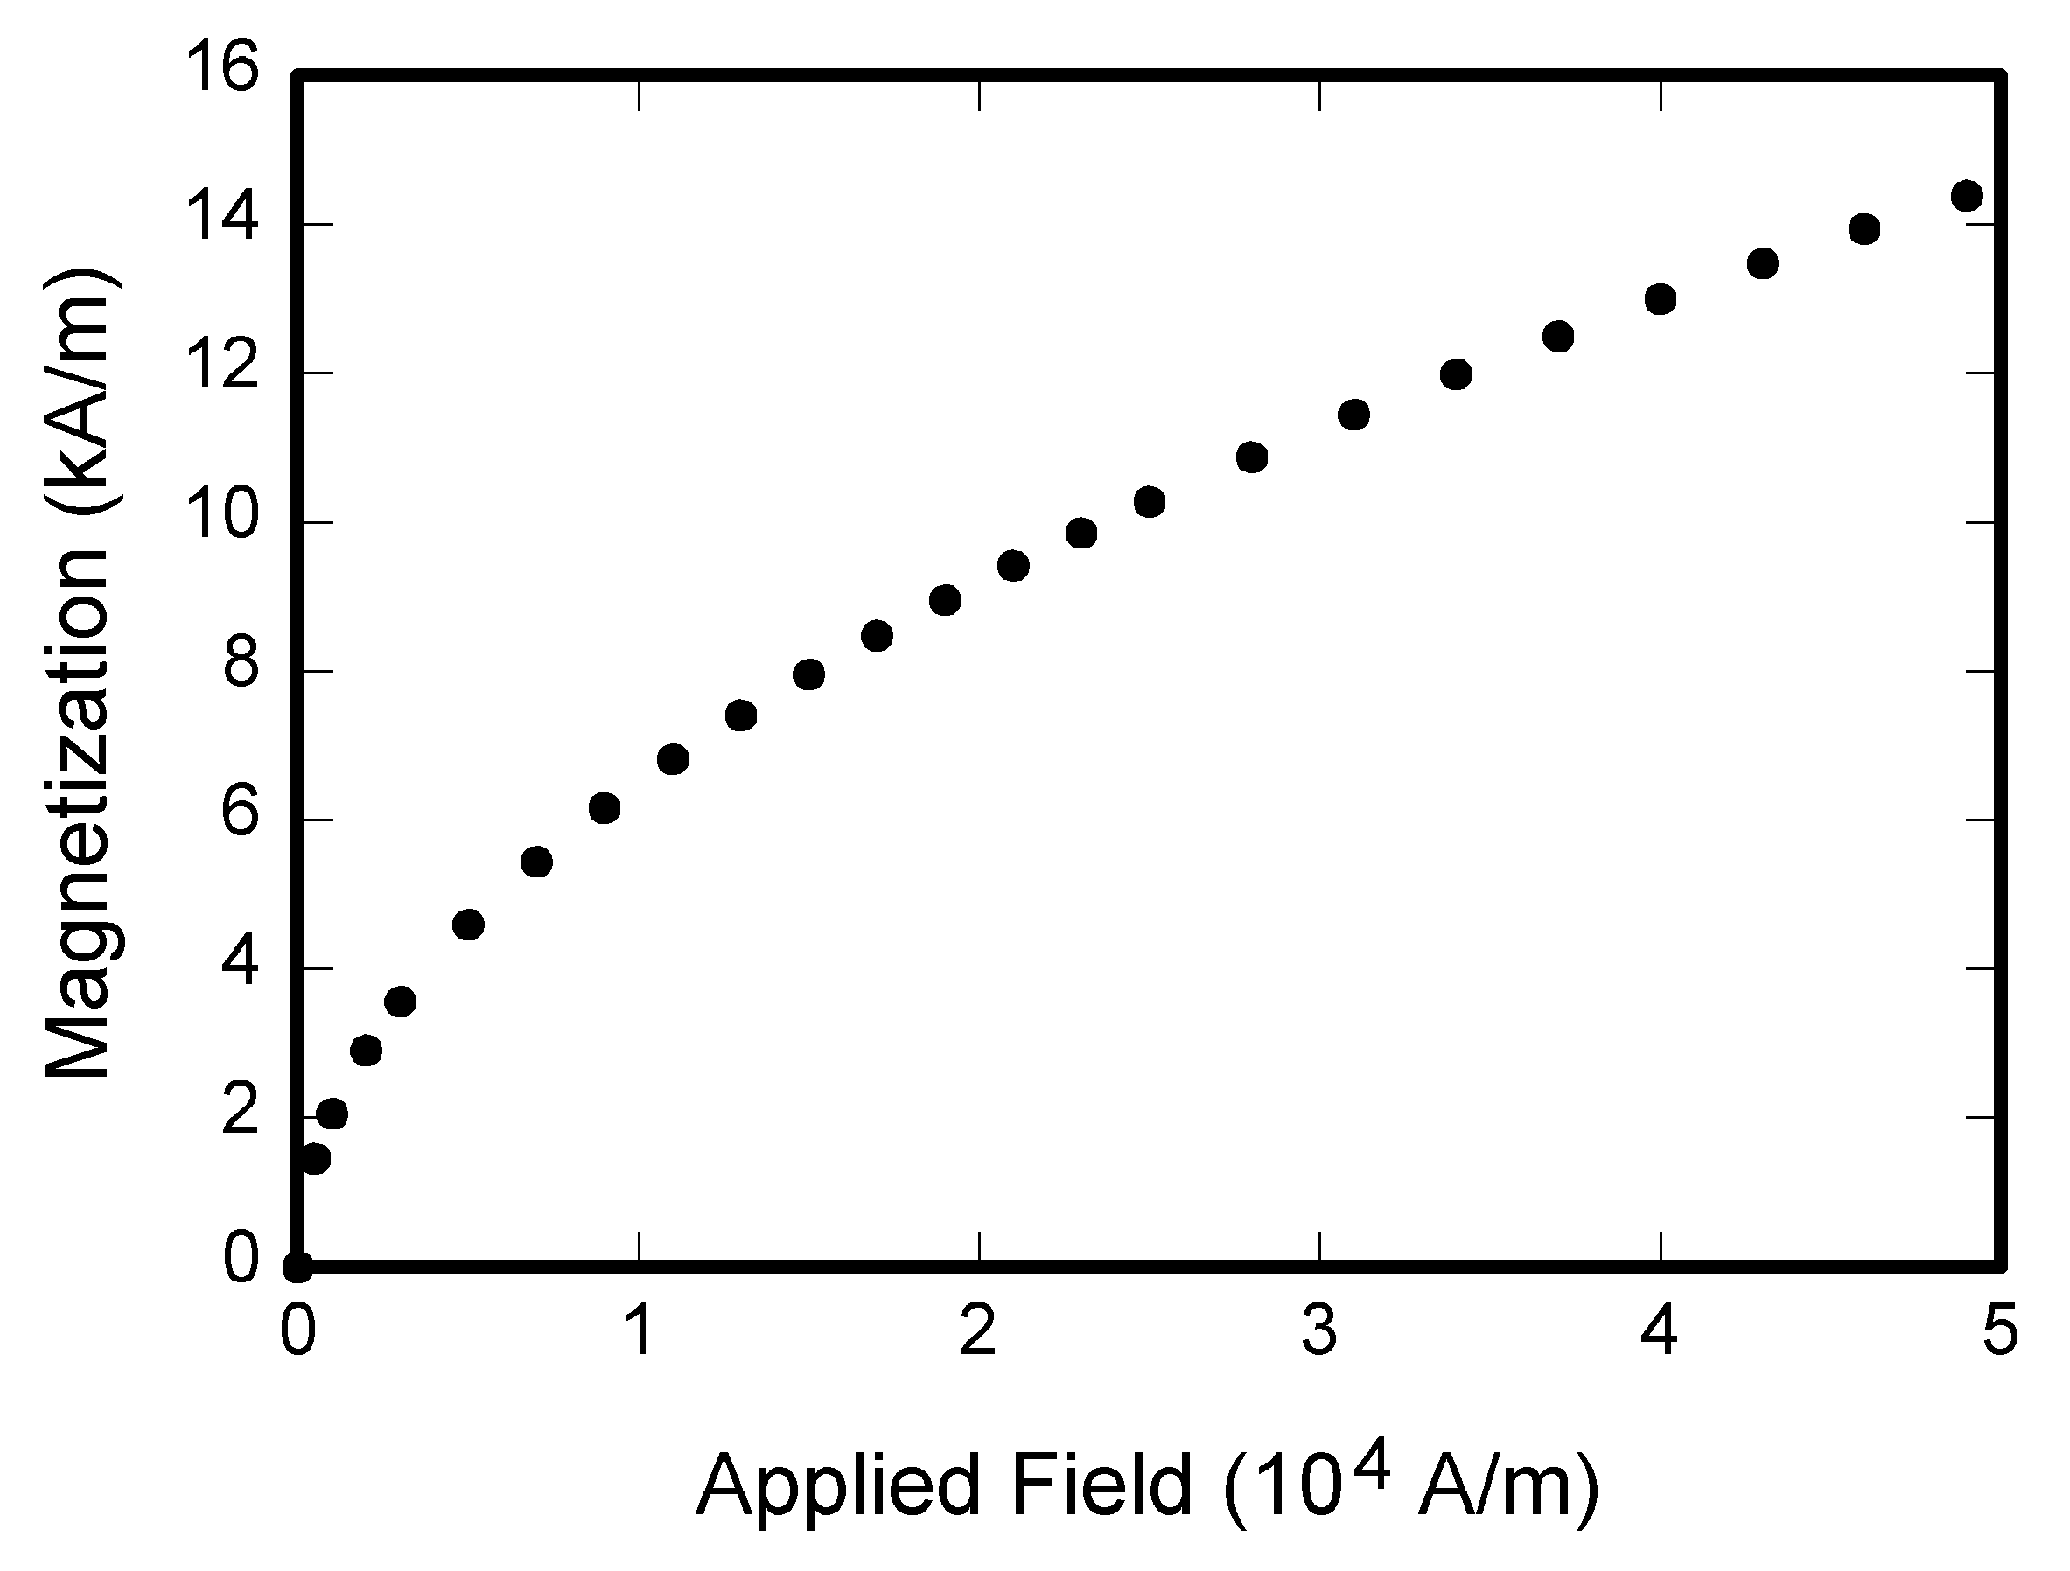
\includegraphics[width=0.85\columnwidth]{figures/fig1.png}
%   \caption{Sample figure placeholder. Replace this with your own figure file.}
%   \label{fig:sample}
% \end{figure}

\section{Results and Discussion}
Insert your results and discussion here. For wide tables or figures, use \verb|table*| or \verb|figure*| carefully, since IEEE two-column layouts restrict where full-width floats can appear.

\section{Conclusion}
Insert the conclusion here.

\appendices
\section{Additional Derivations}
Appendix material can be placed here.

\section*{Acknowledgment}
The authors would like to thank the anonymous reviewers for their constructive comments.

% Option A: direct bibliography, compiles without BibTeX.
\begin{thebibliography}{1}
\bibitem{ref1} A. Author and B. Author, ``A sample article title,'' \emph{IEEE Transactions on Cybernetics}, vol. 54, no. 1, pp. 1--10, 2024.
\bibitem{ref2} C. Author, ``Another sample article title,'' \emph{IEEE Transactions on Automatic Control}, vol. 68, no. 2, pp. 100--112, 2023.
\end{thebibliography}

% Option B: BibTeX. Uncomment the two lines below and use references.bib if desired.
% \bibliographystyle{IEEEtran}
% \bibliography{references}

\end{document}
